\documentclass[11pt]{article}
\usepackage{geometry}
\usepackage{url}
\geometry{letterpaper,textwidth=500pt,textheight=720pt,tmargin=30pt,
            footskip=24pt,headsep=18pt,headheight=14pt}
\RequirePackage{amsmath}
\usepackage{amssymb}
\usepackage{textcase}
\usepackage{soul}
\usepackage{indentfirst}

\newcommand{\eps}{\varepsilon}
\newcommand{\kron}{\otimes}
\DeclareMathOperator{\diag}{diag}
\DeclareMathOperator{\trace}{trace}
\DeclareMathOperator{\tvec}{vec}
\DeclareMathOperator{\rank}{rank}
\DeclareMathOperator{\tspan}{span}
\DeclareMathOperator*{\minimize}{minimize}
\DeclareMathOperator*{\maximize}{maximize}
\DeclareMathOperator{\subjectto}{subject\ to}

\newcommand{\mat}[1]{\boldsymbol{#1}}
\renewcommand{\vec}[1]{\boldsymbol{\mathrm{#1}}}
\newcommand{\vecalt}[1]{\boldsymbol{#1}}

\newcommand{\conj}[1]{\overline{#1}}

\newcommand{\normof}[1]{\|#1\|}
\newcommand{\onormof}[2]{\|#1\|_{#2}}

\newcommand{\MIN}[2]{\begin{array}{ll} \displaystyle \minimize_{#1} & {#2} \end{array}}
\newcommand{\MINone}[3]{\begin{array}{ll} \displaystyle \minimize_{#1} & {#2} \\ \subjectto & {#3} \end{array}}
\newcommand{\OPTone}{\MINone}
\newcommand{\MINthree}[5]{\begin{array}{ll} \displaystyle \minimize_{#1} & {#2} \\ \subjectto & {#3} \\ & {#4} \\ & {#5} \end{array}}

\newcommand{\MAX}[2]{\begin{array}{ll} \displaystyle \maximize_{#1} & {#2} \end{array}}
\newcommand{\MAXone}[3]{\begin{array}{ll} \displaystyle \maximize_{#1} & {#2} \\ \subjectto & {#3} \end{array}}


\newcommand{\itr}[2]{#1^{(#2)}}
\newcommand{\itn}[1]{^{(#1)}}

\newcommand{\prob}{\mathbb{P}}
\newcommand{\probof}[1]{\prob\left\{ #1 \right\}}

\newcommand{\pmat}[1]{\begin{pmatrix} #1 \end{pmatrix}}
\newcommand{\bmat}[1]{\begin{bmatrix} #1 \end{bmatrix}}
\newcommand{\spmat}[1]{\left(\begin{smallmatrix} #1 \end{smallmatrix}\right)}
\newcommand{\sbmat}[1]{\left[\begin{smallmatrix} #1 \end{smallmatrix}\right]}

\newcommand{\RR}{\mathbb{R}}
\newcommand{\CC}{\mathbb{C}}

\providecommand{\eye}{\mat{I}}
\providecommand{\mA}{\ensuremath{\mat{A}}}
\providecommand{\mB}{\ensuremath{\mat{B}}}
\providecommand{\mC}{\ensuremath{\mat{C}}}
\providecommand{\mD}{\ensuremath{\mat{D}}}
\providecommand{\mE}{\ensuremath{\mat{E}}}
\providecommand{\mF}{\ensuremath{\mat{F}}}
\providecommand{\mG}{\ensuremath{\mat{G}}}
\providecommand{\mH}{\ensuremath{\mat{H}}}
\providecommand{\mI}{\ensuremath{\mat{I}}}
\providecommand{\mJ}{\ensuremath{\mat{J}}}
\providecommand{\mK}{\ensuremath{\mat{K}}}
\providecommand{\mL}{\ensuremath{\mat{L}}}
\providecommand{\mM}{\ensuremath{\mat{M}}}
\providecommand{\mN}{\ensuremath{\mat{N}}}
\providecommand{\mO}{\ensuremath{\mat{O}}}
\providecommand{\mP}{\ensuremath{\mat{P}}}
\providecommand{\mQ}{\ensuremath{\mat{Q}}}
\providecommand{\mR}{\ensuremath{\mat{R}}}
\providecommand{\mS}{\ensuremath{\mat{S}}}
\providecommand{\mT}{\ensuremath{\mat{T}}}
\providecommand{\mU}{\ensuremath{\mat{U}}}
\providecommand{\mV}{\ensuremath{\mat{V}}}
\providecommand{\mW}{\ensuremath{\mat{W}}}
\providecommand{\mX}{\ensuremath{\mat{X}}}
\providecommand{\mY}{\ensuremath{\mat{Y}}}
\providecommand{\mZ}{\ensuremath{\mat{Z}}}
\providecommand{\mLambda}{\ensuremath{\mat{\Lambda}}}
\providecommand{\mSigma}{\ensuremath{\mat{\Sigma}}}
\providecommand{\mTheta}{\ensuremath{\mat{\Theta}}}
\providecommand{\mPbar}{\bar{\mP}}

\providecommand{\ones}{\vec{e}}
\providecommand{\va}{\ensuremath{\vec{a}}}
\providecommand{\vb}{\ensuremath{\vec{b}}}
\providecommand{\vc}{\ensuremath{\vec{c}}}
\providecommand{\vd}{\ensuremath{\vec{d}}}
\providecommand{\ve}{\ensuremath{\vec{e}}}
\providecommand{\vf}{\ensuremath{\vec{f}}}
\providecommand{\vg}{\ensuremath{\vec{g}}}
\providecommand{\vh}{\ensuremath{\vec{h}}}
\providecommand{\vi}{\ensuremath{\vec{i}}}
\providecommand{\vj}{\ensuremath{\vec{j}}}
\providecommand{\vk}{\ensuremath{\vec{k}}}
\providecommand{\vl}{\ensuremath{\vec{l}}}
\providecommand{\vm}{\ensuremath{\vec{l}}}
\providecommand{\vn}{\ensuremath{\vec{n}}}
\providecommand{\vo}{\ensuremath{\vec{o}}}
\providecommand{\vp}{\ensuremath{\vec{p}}}
\providecommand{\vq}{\ensuremath{\vec{q}}}
\providecommand{\vr}{\ensuremath{\vec{r}}}
\providecommand{\vs}{\ensuremath{\vec{s}}}
\providecommand{\vt}{\ensuremath{\vec{t}}}
\providecommand{\vu}{\ensuremath{\vec{u}}}
\providecommand{\vv}{\ensuremath{\vec{v}}}
\providecommand{\vw}{\ensuremath{\vec{w}}}
\providecommand{\vx}{\ensuremath{\vec{x}}}
\providecommand{\vy}{\ensuremath{\vec{y}}}
\providecommand{\vz}{\ensuremath{\vec{z}}}
\providecommand{\vpi}{\ensuremath{\vecalt{\pi}}}

\providecommand{\vlambda}{\ensuremath{\vecalt{\lambda}}}
\providecommand{\vdelta}{\ensuremath{\vecalt{\delta}}}
\providecommand{\vtheta}{\ensuremath{\vecalt{\theta}}}


\sodef\allcapsspacing{\upshape}{0.15em}{0.65em}{0.6em}%

\DeclareMathOperator*{\argmin}{arg\,min}
\DeclareMathOperator*{\argmax}{arg\,max}

\makeatletter
\def\maketitle{%
\par
\hrule height 0.75pt\vspace{1ex}
\par\noindent
\begin{minipage}{0.75\textwidth}
\scshape
purdue university $\cdot$ project draft \\
Contrastive Learning to Distentagle Motion
\end{minipage}
\begin{minipage}{0.25\textwidth}
\raggedleft
\MakeTextUppercase{\allcapsspacing{\@title}}\\[0.2ex]
\textit{\@author}\\[0.2ex]
\textit{\@date}
\end{minipage}
\par\vspace{1ex}
\hrule height 1pt
\vspace{2ex}
\par
}
\usepackage{mathtools}
\usepackage{animate}
\usepackage{xcolor}
\usepackage{mdframed}
\usepackage{verbatim}
\newenvironment{jcode}{\mdframed[backgroundcolor=blue!20,linecolor=black,leftmargin=20,rightmargin=20]\verbatim\underline{Julia Code}}{\endverbatim\endmdframed}
\usepackage[ruled,vlined,linesnumbered,]{algorithm2e}
%\usepackage{algorithmic}
\usepackage{parskip}
\newcommand{\algrule}[1][.2pt]{\par\vskip.5\baselineskip\hrule height #1\par\vskip.5\baselineskip}
\usepackage{hyperref,xcolor}
\usepackage{comment}


\makeatother


\usepackage[numbers]{natbib}
\usepackage{subcaption}
\usepackage{wrapfig}

\author{Kent Gauen}
\title{Draft}

\begin{document}

\maketitle

\section{Overview}

The purpose of this project is to disentangle static and dynamic features of an image.
Recent works have show the ability to decouple features and transformations among scenes~\cite{liu2020learning}. Contrastive learning~\cite{chen2020simple,xiao2020should} is a scheme to learn an encoder invariant to a set of user-defined transformations. Further work has demonstrated by modifying the transformation class, the user is able to modify the invariant class of transformations~\cite{xiao2020should}. Based on these ideas, we propose the following project:

Contrastive learning gives us an encoding of the input image $x$, $\tt{enc}_{d}(x)$. We would like to maintain complete information of the original image, while still providing the encoded representation of the image. In other words, we want to take the original image $x$ and apply a representation function $\tt{repr}(x) = \tt{enc}_{c}(x) \cup \tt{enc}_{d}(x)$ where the information contained in encodings are disjoint. Note $\tt{enc}_{d}(x)$ is the \emph{disentangled information} of image $x$. 

We would like to answer the following questions:


\begin{itemize}
\item How can contrastive learning be used to disentangle simple information, e.g. noise, from an image? Can we test the disentangle encoder to generate specified noise?
\item Similar to related work~\cite{xiao2020should}, can we use disentangled representations to capture dynamic lighting?
\item How can we apply contrastive learning to decouple static and dynamic image features?
%\item With our trained $\tt{enc}_{CL}(x) = \tt{enc}_{\text{static}}(x)$ and $\tt{enc}_{DI}(x) = \tt{enc}_{\text{dynamic}}(x)$ , can we use generate new dynamic features on the static scene?
%\item With our trained $\tt{enc}_{CL}(x) = \tt{enc}_{\text{static}}(x)$ and $\tt{enc}_{DI}(x) = \tt{enc}_{\text{dynamic}}(x)$ , can we use generate the next frame in the sequence?
\end{itemize}


\section{Progress Overview}

Complete

\begin{itemize}
\item Contrastive learning: code
\item Contrastive learning: train on cifar-10
\item Contrastive learning: test on cifar-10
\item Image Reconstruction: code
\item Image Reconstruction: train on cifar-10  (10 of +1000 epochs); 
\item Image Reconstruction: test on cifar-10. Did not work well; i did it on color which I am guessing is why it did not work well. Reference only did BW.
\item Image Reconstruction: train on cifar-10 black and white  (10 of +1000 epochs); (i want to move on to disentanglement so I left this)
\end{itemize}

In progress

\begin{itemize}
\item Disentanglement Network: code
\item Write down the decoupling mechanism for noisy images
\item Disentanglement Network: train on mnist
\item Disentanglement Network: test on mnist
\end{itemize}


To do

\begin{itemize}
\item Disentanglement Network: train on cifar-10
\item Disentanglement Network: test on cifar-10
\item Identify more related work
\end{itemize}

Maybe To do 

\begin{itemize}
\item Image Reconstruction: train on face dataset
\item Image Reconstruction: test on face dataset
\item Write down the decoupling mechanism for noisy images
\item Disentanglement Network: code
\item Disentanglement Network: train on cifar-10
\item Disentanglement Network: test on cifar-10
\item Identify more related work
\end{itemize}

\section{Related Work}


Recent work on contrastive learning has demonstrated the ability to learn unsupervised representations of images useful for downstream tasks such as classification and localization~\cite{chen2020simple}. This paper outlines the simple generalization of the NT-Xent loss function. We validate the loss function and explore the impact on training from moving from pairs of transformations to a collection of size $N$. 

Recent research on learning invariant representations in deep learning networks has lead to state-of-the-art performance for image reconstruction~\cite{xia2019training}. This method of learning invariances depends on collecting a diverse set paired noisy images with a known noise mechanism (but possibly unknown parameters). Our proposed method does not require knowing the noise mechanism or parameters. By disentangling the static image and transformation operation, we can apply the transformation from one image to another with no knowledge of the noise mechanism. 
We validate our method on image reconstruction tasks and observed state-of-the-art performance compared to previous methods.


Recent work on disentangling static and dynamic images has shown several results. Recently~\cite{liu2020learning} proposed a method to decompose the time-varying illumination and static scene components. While our method also utilizes swapping with encoders and decoders, this paper uses the contrastive learning loss function compared to the $L_1$ loss function. We experimentally demonstrate the significance of the contrastive learning loss function in Section~\ref{subsec:gnt_xent_illumination}


\section{Disentangling Model for Semantically Invariant Transformations}

This method utilizes encoders, a decoder, and swapping to disentangle static and dynamic scene components from a collection of input images. The relationships between the encoders, decoder, and swapping is shown in Figure~\ref{fig:disent_losses_invariant}(a) and equation~\ref{eq:repr}. The input is assumed to be a transformed image $t_i(\vx)$. This transformed image is the input to both the static encoder ${\tt enc_{c}}$ or the dynamic encoder ${\tt enc_{d}}$. The representations of the dynamic encoder is decoded with each static representation and then decoded once more. This ``swapping-propogation'' allows us to use the contrastive learning loss function along the final decoded representations. The static components utilize information from both the first and second steps of decoding. In Section~\ref{sec:gen_nt_xent}, we explore the impact of the second decoding step on the learned model and static representations. This method trains the static encoder to be invariant to non-semantic changes of the image, and trains the dynamic encoder to be invariant to the static image semantics. Thus the information the encoders capture is disjoint. To ensure the representations are complete, we also include an image construction loss. This image reconstruction loss forces the embeddings to retain semanic information of the image.

\begin{figure*}[h]
  \begin{subfigure}[b]{0.195\textwidth}
    \centering
    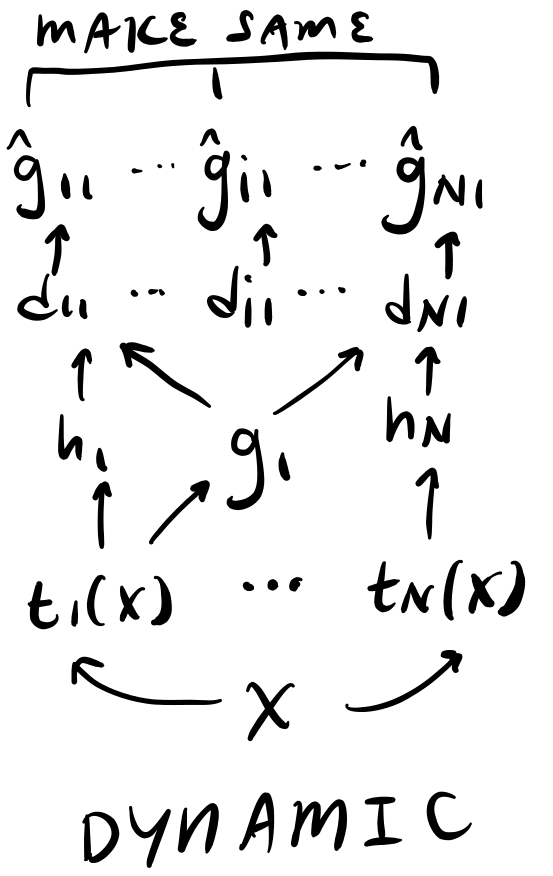
\includegraphics[height=1.8in]{figs/disentangle_loss_dynamic}
    \caption{}
  \end{subfigure}
  ~
  \begin{subfigure}[b]{0.395\textwidth}
    \centering
    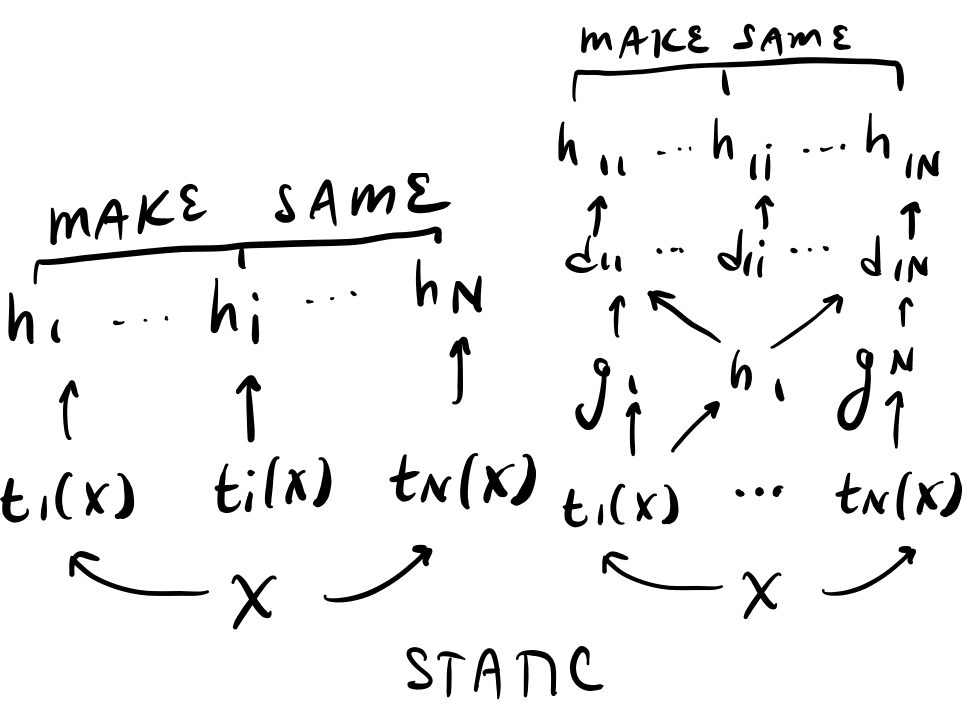
\includegraphics[height=1.8in]{figs/disentangle_loss_static}
    \caption{}
  \end{subfigure}%
  ~
  \begin{subfigure}[b]{0.395\textwidth}
    \centering
    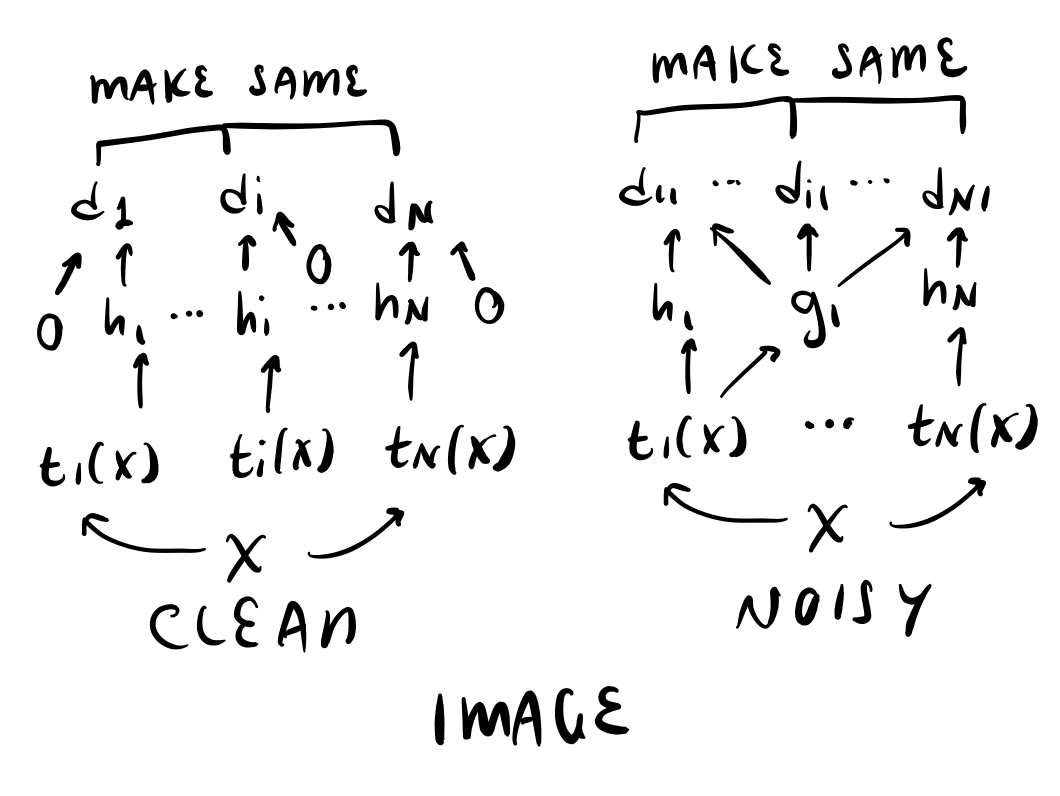
\includegraphics[height=1.8in]{figs/imgrec_loss}
    \caption{}
  \end{subfigure}%
  \caption{This figure shows the structure of the disentanglement framework for semanically invariant transformations $t_i$. The diagram in figure (a) shows the disentanglement loss and figure (b) shows the image reconstruction loss. Both losses are achieved through encoding statics and dynamics, swapping embeddings, and decoding the swapped values.}
  \label{fig:disent_losses_invariant}
\end{figure*}

When transformation $t_i$ applied is applied to the input image $\vx$, $t_i(\vx)$, the encoded static representation is $\vh_i \in \mathbb{R}^{n_{enc}} $ and encoded dynamic representation is $\vg_i \in \mathbb{R}^{n_{enc}}$. The decoder can accept any pair of encodings. When decoding using the static representation from transformation $t_i$ and dynamic representation from transformation $t_j$, the decoded vector is denoted $\vd_{i,j}$. The ability for the decoder to swap static and dynamic embeddings is the key of our proposed method. This allows us to propogate apply the transformations to the static representations through decoding, encoder the image dynamics, and apply the contrastive learning loss.


We propose five different loss functions. The first loss the to learn dynamic scene encoding. This loss is shown in Figure~\ref{fig:disent_losses_invariant}(a). For each content embedding, we decode with a fixed dynamic embedding. Thus the resulting image's dynamics can be futhur encoded and should all be equal. We apply a generalized nt-xent (gNT-Xent) loss function to make all the representations agree. Similar to contrastive learning, the negative samples are the other images in the batch. The projection operation is applied to the encoded representations before the cosine similarity is computed.

The next two loss functions learn the static scene encoding. The first static scene loss is simply a simple generalization of the NT-Xent loss function~\cite{chen2020simple} and is depicted in Figure~\ref{fig:disent_losses_invariant}(b) on the left-hand side. This is the contrastive learning loss function applied to $N$ inputs rather than a pair of inputs. In Figure~\ref{fig:disent_losses_invariant}(b) on the right, we show the second staic scene loss applied after a step of decoding and encoding. The purpose of this loss is to influence the the gradient of the decoder. We conjecture this second static encoding loss will decrease training time by providing more information each update. Again, the projection operation is applied to the encoded representations before the cosine similarity is computed.
 
The final two loss functions are for image reconstruction. In Figure~\ref{fig:disent_losses_invariant}(c), we set the zero vector to indicate the output image should contain only the semantic information. Thus all reconstructed images should contain only the original image, and we apply the contrastive learning loss in image space. We do not compare the reconstructed images to the original input image to simulate not having access to the groundtruth image. We demonstrate the impact of including a loss term comparing to the original image to the clean reconstructed images in Section~\ref{subsec:disent_mnist_denoising}. In Figure~\ref{fig:disent_losses_invariant}(c) on the right, we show the noisy image reconstruction loss. When the decoder uses the embeddings from the same transformation, the decoded image should be the same as the original image: $\vd_{i,i} \approx t_i(\vx)$. 


\begin{align}\label{eq:repr}
  \vh_i &= {\tt enc_c}(t_i(\vx)) &  \vg_i &= {\tt enc_d}(t_i(x)) &  \vd_{i,j} &= {\tt dec}(\vh_i,\vg_j)
  \\\nonumber
  \hat{\vh}_{i,j} &= {\tt enc_c}(\vd_{i,j}) & \hat{\vg}_{i,j} &= {\tt enc_d}(\vd_{i,j}) & \vd_i &= {\tt dec}(\vh_i,0)
\end{align}

The generalized contrastive learning loss for a tensor $\mZ = (N,M,P)$ with $N$ transformations and batch size $M$ is given by the following:

\begin{align}
  l_{i,j}(\mZ)
  =
  -\log
  \frac{
  \exp\left(\text{sim}(\vz_i,\vz_j)/\tau\right)
  }{
  \sum^{N*M}_{k=1}\mathbbm{1}_{k \in \mathcal{D}_{(N,M)}}\exp\left(\text{sim}(\vz_i,\vz_k)/\tau\right)
  }
\end{align}

We let $\mathcal{D}_{(N,M)}$ be the index set for samples different from sample $i$ when $\mZ$ has $N$ different transformations and a batch size of $M$. Similar to~\cite{chen2020simple}, we compute the loss over all positive pairs $(i,j)$ and $(j,i)$. We term this loss the \emph{Generalized NT-Xent}.  We show experimentally how this generalized version compares with the original \emph{NT-Xent} loss function in Section~\ref{sec:gen_nt_xent}. To compute the loss functions, we aggregate the encoded representations such that along the first dimension all representations should have the same values.

\begin{align}\nonumber
  \mG_{\text{swap}}^i &= (\vg_1,\hat{\vg}_{2,i},\ldots,\hat{\vg}_{N,i})                                 &
  \mH_{\text{swap}}^i &= (\vh_1,\hat{\vh}_{i,1},\ldots,\hat{\vh}_{i,N}) & \mH_{\text{self}} &= (\vh_1,\vh_2,\ldots,\vh_N)
   \\\nonumber                          
  \mD_{\text{noisy}}^i &= (\vd_{1,i},\ldots,\vd_{N,i})
  &                     
  \mD_{\text{clean}} &= (\vd_1,\ldots,\vd_N)
\end{align}

The explicit formula for computing the contrastive learning loss is given as

\[
  L_h = \gamma_h \sum_{i=1}^N {\tt gNtXent}(\vh_i,\vh_{i,1},\ldots,\vh_{i,N})
\]

\[
  {\tt gNtXent}(\vh_i,\hat{\vh}_{i,1},\ldots,\hat{\vh}_{i,N})
  =
  {\tt gNtXent}(\vz_1,\vz_2,\ldots,\vz_{N+1})
  =
  \sum_{i=1}^{N+1} \sum_{j=1}^{N+1} \mathbbm{1}[(i,j) \in \mathcal{V}(N+1,M)] l_{i,j}
\]

With the first dimension size $N+1$ being representation with the same encoding and the second dimension size $M$ being the batch size, supplying negative samples for the contrastive learning loss.

\section{Disentangling Model for Semantically Varying Transformations}

\begin{figure*}[h]
  \begin{subfigure}[b]{0.33\textwidth}
    \centering
    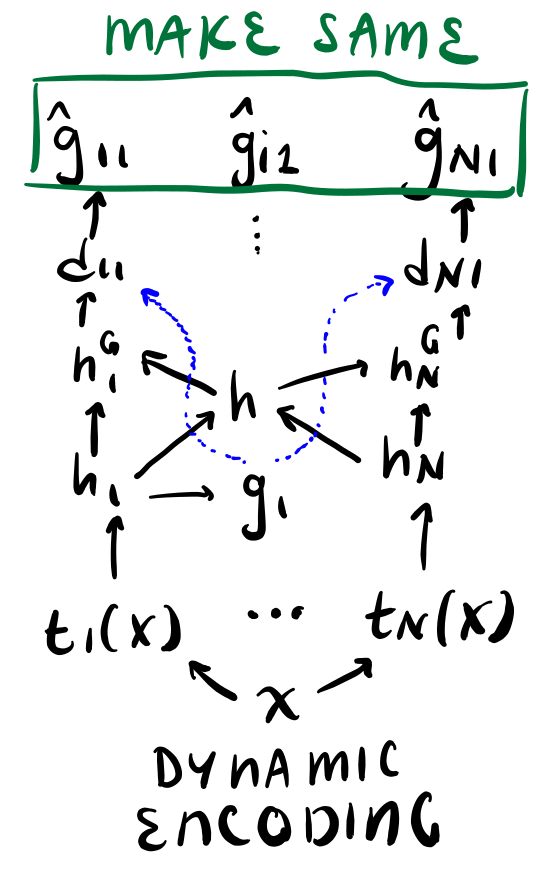
\includegraphics[height=1.8in]{figs/disentangle_loss_dynamic_varying_ti}
    \caption{}
  \end{subfigure}
  ~
  \begin{subfigure}[b]{0.33\textwidth}
    \centering
    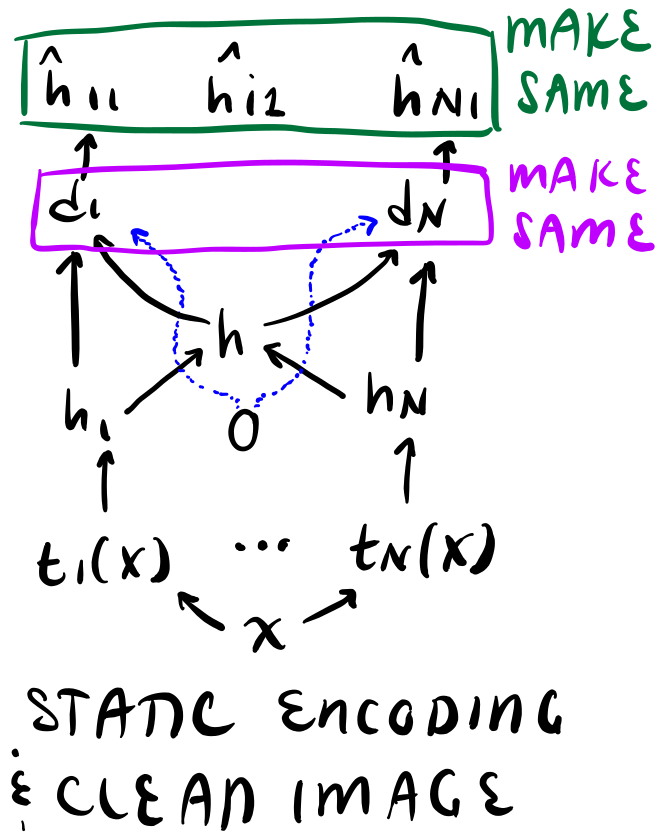
\includegraphics[height=1.8in]{figs/disentangle_loss_static_clean_varying_ti}
    \caption{}
  \end{subfigure}%
  ~
  \begin{subfigure}[b]{0.33\textwidth}
    \centering
    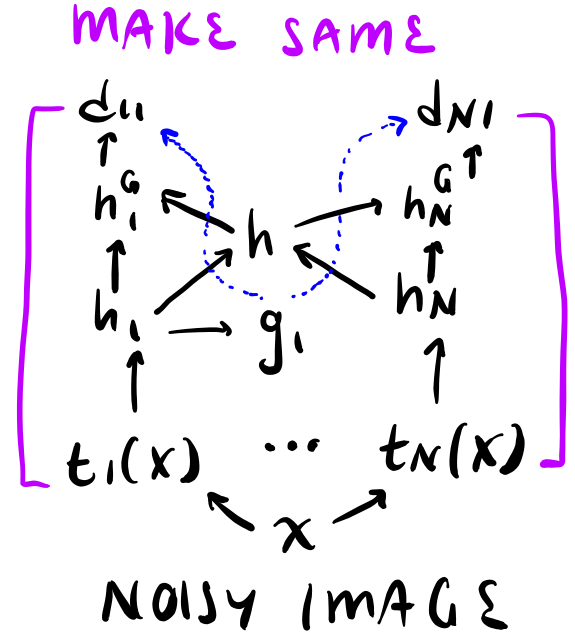
\includegraphics[height=1.8in]{figs/disentangle_loss_noisy_varying_ti}
    \caption{}
  \end{subfigure}%
  \caption{This figure shows the structure of the disentanglement framework for semantically varying transformations $t_i$. This is an adjusted version of semanically invariant transformations to allow encoded representations for each transformed image $t_i(\vx)$ to vary with each transformation.}
  \label{fig:disent_losses_varying}
\end{figure*}


Figure~\ref{fig:disent_losses_varying}(c) including the $\vg_i$ term: We can think of $\vh = {\tt GCN}(\vh_1,\ldots,\vh_N)$ as scene, $\vh_k^G$ as the viewpoint $k$, $\vg_i$ as ``additional noise'', and $\vd_{i,1}$ as the decoded image with ``additional noise'' from $i$. The video $\vh$ pans across to create the view points but the camera picks up noise.

Figure~\ref{fig:disent_losses_varying}(c) without the $\vg_i$ term: We can think of $\vh = {\tt GCN}(\vh_1,\ldots,\vh_N)$ as static component and $\vh_k^G$ as the dynamic component with $\vd_{i,1}$ as the decoded noisy image and $\vh$ as the decoded clean image. This also gives one decoder and one encoder.

In Figure~\ref{fig:disent_losses_varying}, say we remove the second encoder. This is nice since we handle dynamics through the graphconv operations. But then the question is: how do we include a contrastive learning term for the dynamics of the image? In Figure~\ref{fig:disent_losses_varying}(a) shows how the second encoder gives us a ``plug-and-play'' ability. We might be able to resolve this problem by identifying a smart ``aggregate'' function. For example...

GIN~\cite{wu2020comprehensive} identifies the following general functions used in graph convolution:

\begin{align}
  a_v^{(k)}
  &=
  {\tt AGGREGATE}^{(k)}
  \left(\left\{
  h_u^{(k-1)} : u \in \mathcal{N}(v)
  \right\}\right),
  &
  h_v^{(k)}
  &=
  {\tt COMBINE}^{(k)}
  \left(
  h_v^{(k-1)},a_v
  \right)
\end{align}

for $h_v^{(k)}$ is the feature vector of node $v$ at the $k$-th iteration/layer. 



\newpage

\section{Generalized NT-Xent Loss}\label{sec:gen_nt_xent}

we explore the impact of the second decoding step on the learned model and static representations.

This section runs experiments demonstrating how generalizing the NT-Xent loss changes the (i) how learning runs over epochs, (ii) how this changes for different types of transformations, (iii) new tasks (just with contrastive learning setup) the generalized version can complete the pair-wise contrastive learning cannot complete.



\subsection{Image Denoising}\label{subsec:gnt_xent_denoising}

We run image denoising experiments by adding random Gaussian noise to a ``clean'' images $N$ times. We compare the results of image denoising compared with~\cite{xia2019training,metzler2016denoising,li2013efficient}. We do 

\subsection{Dynamic Illumination}\label{subsec:gnt_xent_illumination}

\section{Disentangling Gaussian Noise, Random Noise Blocks, and Motion with MNIST Data}\label{sec:disent_mnist}

Note, we can re-do this experiment set of something more complicated once we demonstrate feasibility with something small and simple like MNIST.

This experiment demonstrates the models ability to decouple the static background image from dynamic changes across different images.

For two different types of dynamics, we explore the impact of batch size, noise block size, and number of noisy images during learning.

For both experiments, we also use tsne to plot the relationship among the dynamic encodings. We expect to capture spatial location within the image and see that ``top left'' noise blocks are grouped together while ``bottom right'' noise blocks are far away and aggregated together.


\subsection{Image Denoising}\label{subsec:disent_mnist_denoising}

We run image denoising experiments by adding random Gaussian noise to a ``clean'' images $N$ times. We compare the results of image denoising compared with our \emph{Generalized NT-Xent results} and related literature~\cite{xia2019training,metzler2016denoising,li2013efficient}.

Also, we demonstrate the impact of including a loss term comparing to the original image to the clean reconstructed images.

\subsection{Random Noise Blocks}\label{subsec:disent_mnist_noise_block}

We randomly overlay a block of noise covering about 20\% of the image $N$ times. 

We explore the classification quality of the static embeddings after training.

For dynamic embeddings, we fit a regression model to the center of the noisy patch created by the decoder fixing the dynamic encoding  for each static encoder. We evaluate the quality on a generated test set.

We qualitatively demonstrate the ability to use the static encoding from one image and dynamic encoding of another to create the original noisy image from the dynamic component. E.g. We compare (i) $\vd_{i,j}$ with $t_j(\vx)$ and (ii) $\vd_{i}$ with $\vx$.

\subsection{Moving Digits}\label{subsec:disent_mnist_motion}

We qualitatively demonstrate the ability to use the static encoding from one image and dynamic encoding of another to create the original noisy image from the dynamic component. E.g. We compare (i) $\vd_{i,j}$ with $t_j(\vx)$ and (ii) $\vd_{i}$ with $\vx$.


\newpage

\bibliographystyle{abbrvnat}
\bibliography{ref}


\end{document}


% auto generate a title
% \AtBeginDocument{\maketitle}
